\documentclass{article}
\usepackage{algorithm}
\usepackage{algpseudocode}
\usepackage{graphicx}
\graphicspath{ {images/} }
\usepackage{amssymb}
\usepackage{adjustbox}
\usepackage{placeins}
\usepackage{geometry}
\geometry{tmargin = 1in}

\begin{document}
        
\begin{algorithm}[ht]
\caption{Reverse-Cuthill-McGee Redordering}\label{RCM}
\begin{algorithmic}
\Procedure{RCM}{$mesh$}
    \State node\_label $\gets$ num\_nodes$ + 1$
    \State face\_label $\gets$ num\_faces$ + 1$
    \State Queue q
    \State MeshEntity start\_entity $\gets$ \Call{getStartNode}{mesh}
    \State q.enqueue(start\_entity)
    \While{q.size() $> 0$}
        \State MeshEntity entity = q.dequeue()
        \State Node node = entity.getNode()

        \If{\textbf{not} node.isLabeled}
            \State node.setLabel(label\_node)
            \State label\_node $\gets$ label\_node$ - 1$
        \EndIf

        \If{entity \textbf{is} MESH\_VERTEX }
            \State \Comment{ label neighboring faces and specific edge nodes}
            \State MeshEntity current\_vertex $\gets$ entity \Comment{relabel for clarity}

            \For{$ii = 1$ \textbf{to} vertex.numEdges()}
                MeshEntity edge $\gets$ vertex.edge(ii)
                \For{$jj = 1$ \textbf{to} edge.numFaces()}
                    \State MeshEntity face $\gets$ edge.face(jj)
                    \If{\textbf{not} face.isLabeled()}
                        \State face.setLabel(face\_label)
                        \State face\_label $\gets$ face\_label$ - 1$
                    \EndIf
                    \If{face.hasNode()}
                        \If{\textbf{not} face.getNode().isLabeled()}
                            \State q.enqueue(face)
                        \EndIf

                    \EndIf
                \EndFor

                \State MeshEntity other\_vertex $\gets$ edge.getOtherVertex()
                \If{edge.hasNode()}
                    \If{ other\_vertex.isLabeled() \textbf{or} queue.inQueue(other\_vertex) \textbf{and not} edge.isLabeled() }
                        \State edge.getNode().labelNode(node\_label)
                        \State node\_label $\gets$ node\_label$ - 1$
                    \Else
                        \State q.enqueue(edge)
                        \State list.push\_back(other\_vertex)
                    \EndIf
                \Else
                    \If{\textbf{not} other\_vertex.isLabeled()}
                        \State list.push\_back(other\_vertex)
                    \EndIf
                \EndIf
            \EndFor

\algstore{myalg}
\end{algorithmic}
\end{algorithm}

\begin{algorithm}
\begin{algorithmic}
\algrestore{myalg}

            \State \Call{enqueueList}{q, list}
            \State list.clear()

        \EndIf

    \EndWhile
\EndProcedure
\State
\Procedure{getStartNode}{$mesh$}[t]
    \State\Comment{for $M^{0}_{i} \in [M^{0}]$ \textbf{and}\  $M^{0}_{i} \sqsubset G^{0}$ find min $M^{0}_{i}\{M^{1}\}$}
    \State min\_order $\gets$ INTMAX
    \State MeshEntity best\_vertex
    \State MeshEntity entity $\gets$ mesh.getFirstVertex()
    \While{vertex $\gets$ mesh.getNextVertex()}
        \If{mesh.getModelType(vertex) == MODEL\_VERTEX}
            \State adjacency\_size $\gets$ mesh.getAdjacent()
            \If{adjaceny\_size $<$ min\_order}
                \State min\_order $\gets$ adjaceny\_size
                \State best\_vertex $\gets$ entity
            \EndIf
        \EndIf
    \EndWhile
    \State\Return best\_entity
\EndProcedure
\State
\Procedure{enqueueList}{queue, list}
    \For{item \textbf{in} list}
        \If{item \textbf{is not in} queue}
            \State queue.enqueue(item)
        \EndIf
    \EndFor
\EndProcedure

\end{algorithmic}
\end{algorithm}

\FloatBarrier

\begin{figure}[ht]
\caption{Original labeling of entities by memory address order}
\adjustbox{trim= {0.2\width} {0} {0.2\width} {0}, clip}
{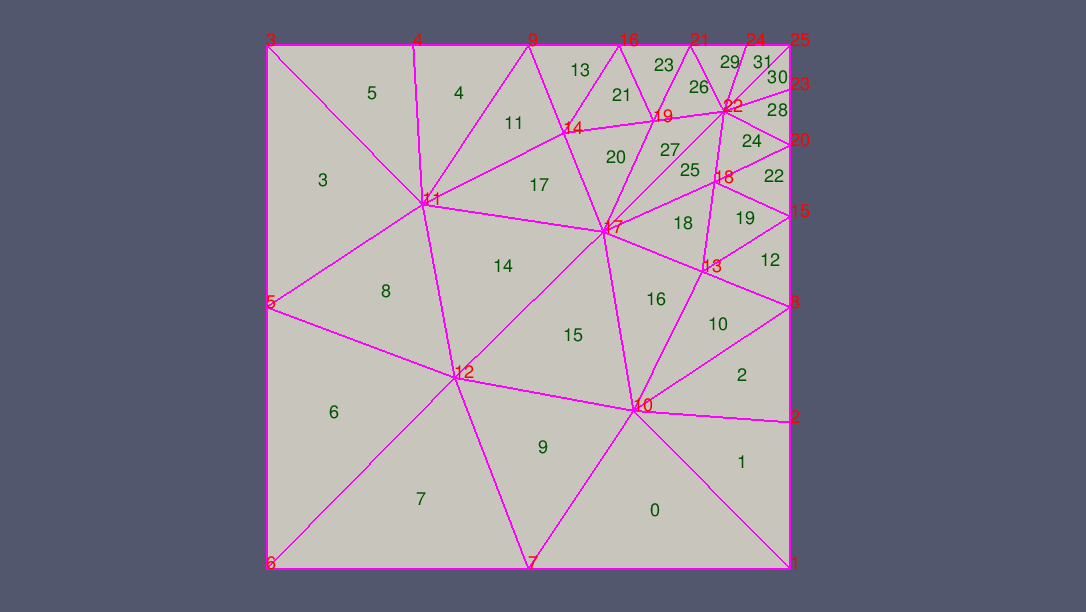
\includegraphics[width = 15cm ]{pre_b}}
\centering
\end{figure}

\begin{figure}[h]
\caption{Reordering with Reverse Cuthill-McGee}
\adjustbox{trim= {0.2\width} {0} {0.2\width} {0}, clip}
{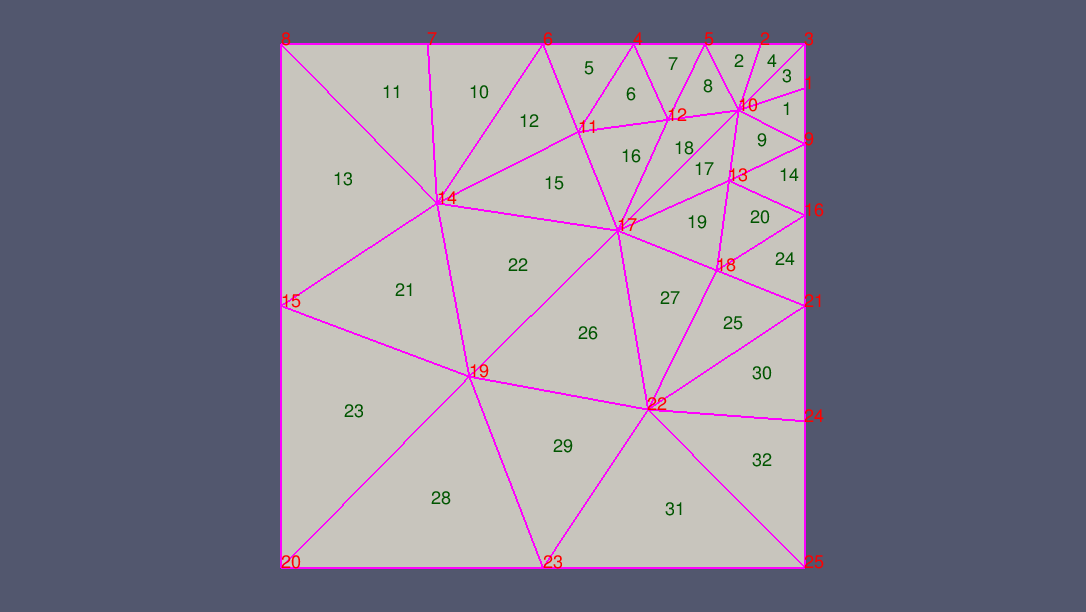
\includegraphics[width = 15cm ]{post_b}}
\centering
\end{figure}

\begin{figure}[ht]
\caption{Original labeling of entities by memory address order}
\adjustbox{trim= {0.2\width} {0} {0.2\width} {0}, clip}
{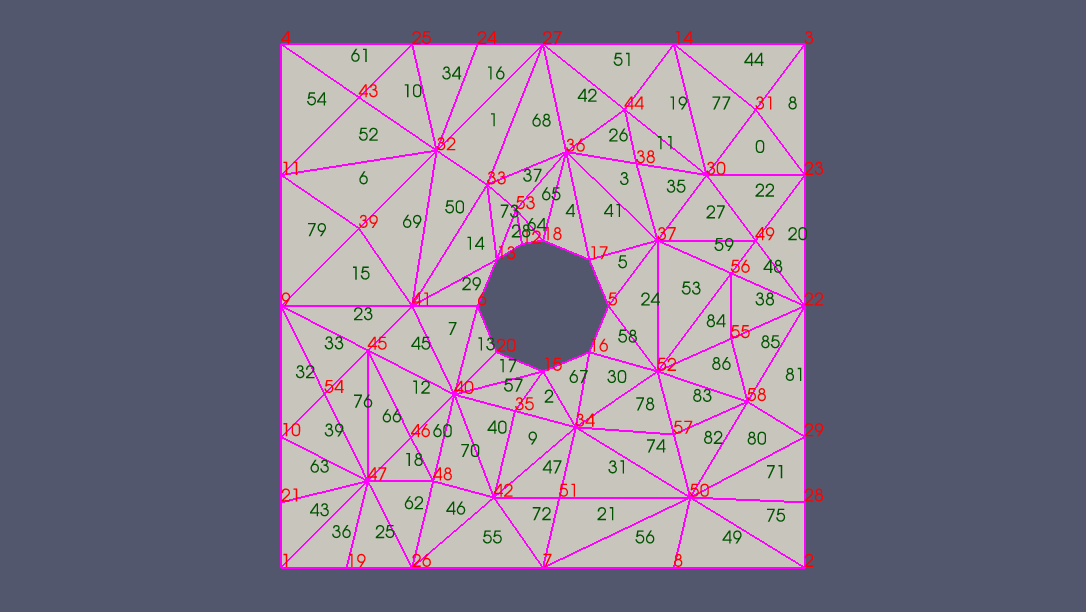
\includegraphics[width = 15cm ]{pre_c}}
\centering
\end{figure}

\begin{figure}[h]
\caption{Reordering with Reverse Cuthill-McGee}
\adjustbox{trim= {0.2\width} {0} {0.2\width} {0}, clip}
{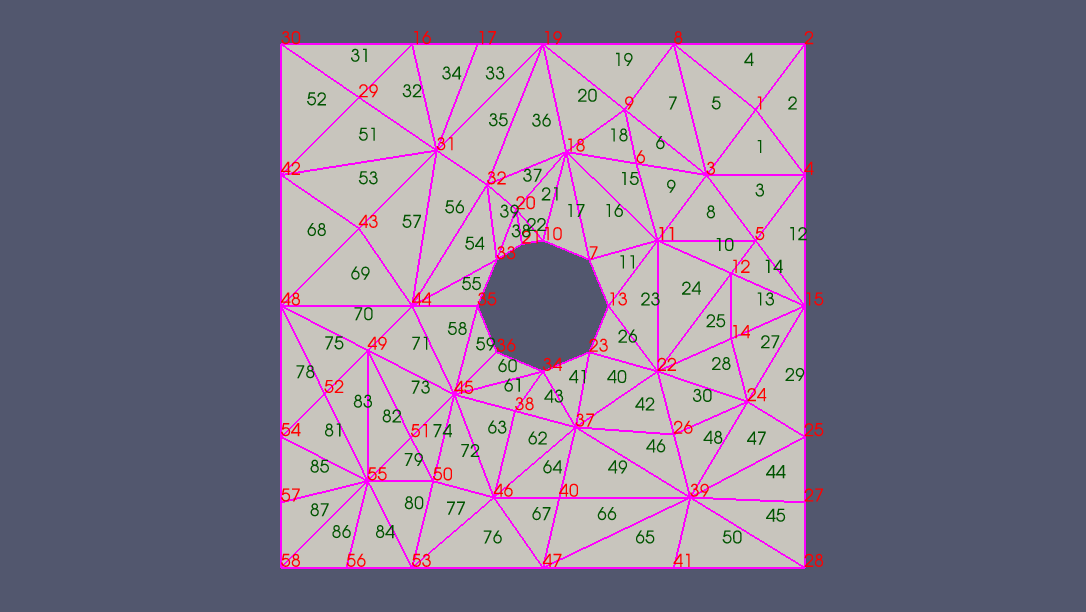
\includegraphics[width = 15cm ]{post_c}}
\centering
\end{figure}

\begin{figure}[ht]
\caption{Original labeling of entities by memory address order}
\adjustbox{trim= {0.2\width} {0} {0.2\width} {0}, clip}
{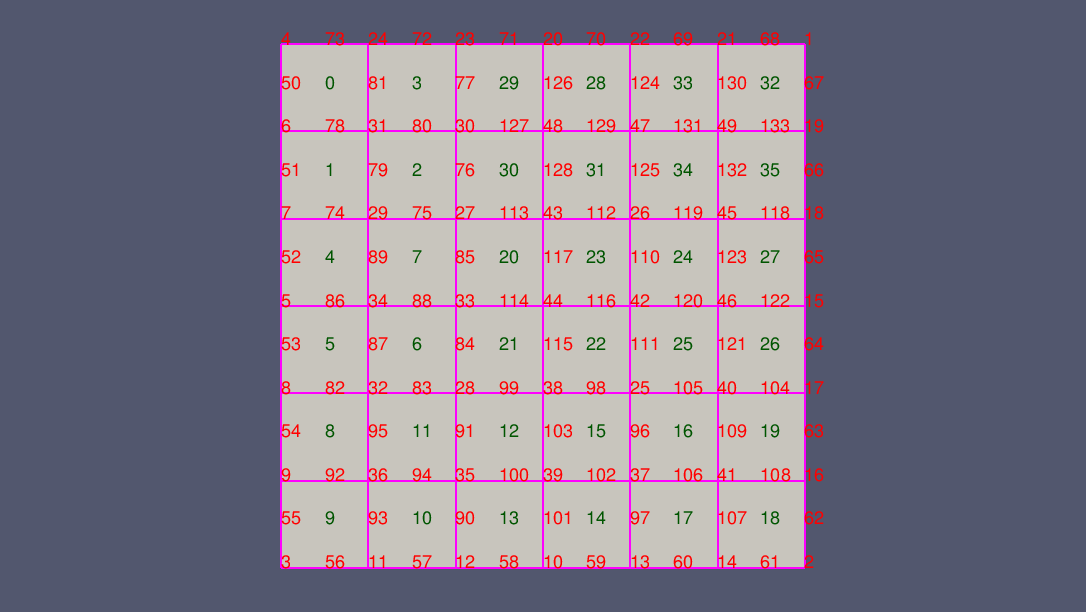
\includegraphics[width = 15cm ]{pre_a}}
\centering
\end{figure}

\begin{figure}[h]
\caption{Reordering with Reverse Cuthill-McGee}
\adjustbox{trim= {0.2\width} {0} {0.2\width} {0}, clip}
{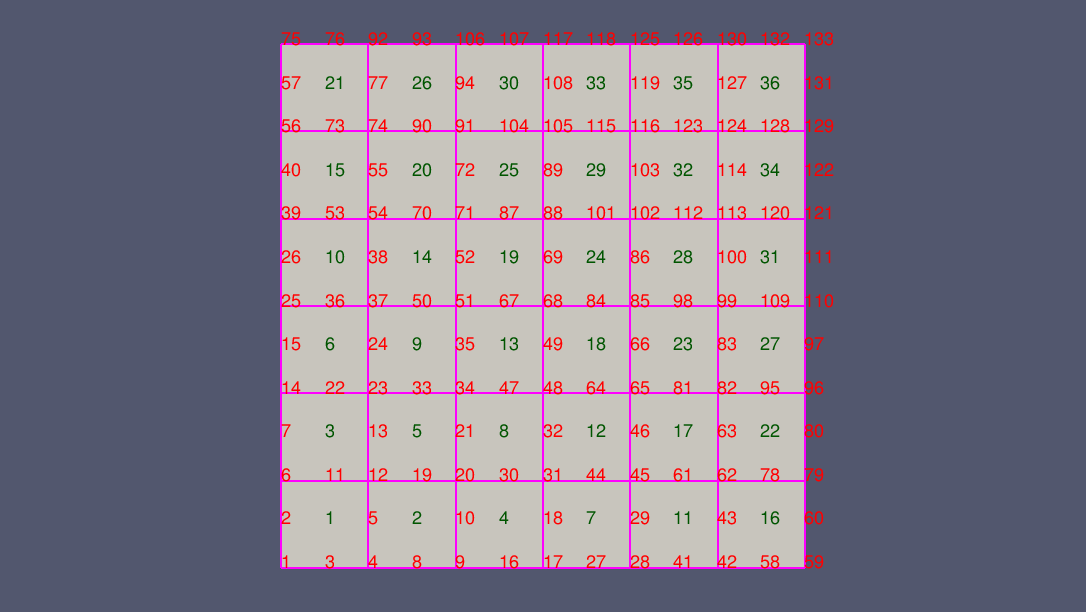
\includegraphics[width = 15cm ]{post_a}}
\centering
\end{figure}

\end{document}
